\documentclass[11pt]{article}

\usepackage[margin=1in]{geometry}
\usepackage{microtype}
\usepackage{multicol}
\usepackage{amsmath}
\usepackage{graphicx}
\usepackage{booktabs}
\usepackage[hidelinks]{hyperref}

\setlength{\emergencystretch}{1.5em}

\newcommand{\natex}{\texttt{natex}}

\title{Natural Experiments in the Public Record of AI:\\ A Systematic Survey}
\author{Hauke Hillebrandt\thanks{University College London. Email:
\texttt{ucjthhi@ucl.ac.uk}. This paper and the underlying \natex{} software were
prepared with substantial assistance from Anthropic's Claude models; the author
reviewed the analyses and text and is responsible for all remaining errors.
Latest version: \url{https://haukehillebrandt.github.io/natex/}.}}
\date{July 2026 \\ \small analysis passes of record: 2026-07, \natex{} v0.2.0;
all stochastic steps seeded}

\begin{document}

\maketitle

\begin{abstract}
\noindent The public record of AI --- benchmark scores, adoption surveys,
capital expenditure, chip stocks, model registries, crowd-sourced battle
streams --- is full of dated events that are claimed, usually by eye, to have
bent some curve. We survey a systematic attempt to test such claims with
formal quasi-experimental designs, run and validated by the open-source
\natex{} toolkit: 17 dataset--design analyses carried to a verdict and 15
more triaged and excluded for cause, each subjected to a mandatory
falsification battery (specification grids, shifted-cutoff placebo grids,
placebo units and outcomes, density and covariate checks, pinned controls,
honest refusals). Eight findings are selected here by credibility and
interest. Three are credible: the 2025 BTOS questionnaire rewording moved
measured US business AI adoption by $+6.0$ pp ($4.7\times$ the largest of 49
placebos), the October-2023 export controls bent China's legal AI-chip stock
by $-0.3$ to $-0.56$ log-units/yr against every control group (25/25
specifications, loophole-round placebo null), and GPQA-Diamond's slope
$2.4\times$'d at o1-preview with a clean placebo grid (0/7). One is moderate:
an 83\% post-Act deficit of models just above the EU AI Act's
$10^{25}$-FLOP line. Two are first-class negatives: the Epoch Capabilities
Index shows no kink at o1 in a design with demonstrated power, and the
sycophantic GPT-4o build won zero opponent-adjusted votes on LMArena. And two
are cautionary: a sharp January-2025 adoption acceleration that cannot be
attributed to DeepSeek-R1, and a hyperscaler capex ``kink'' at ChatGPT whose
nominal $p = 4\times10^{-6}$ collapses to a placebo-calibrated $0.125$. Across
the corpus, roughly half of the nominally significant estimates die in the
battery --- on short, serially dependent, composition-churned series, the
falsification battery is not a robustness appendix; it is the analysis.
\end{abstract}

\section{Introduction}\label{sec:intro}

Public discussion of AI progress and AI policy runs on dated trend breaks.
Reasoning models ``changed the slope'' of capabilities; ChatGPT ``ignited''
the datacenter buildout; export controls ``choked'' China's compute; DeepSeek
``bent'' the adoption curve; the EU AI Act ``chilled'' large training runs.
Each claim names an event, a series, and a shape --- which makes each one a
candidate for a formal quasi-experimental design: a regression discontinuity
or kink at a known cutoff \cite{card2015,hausman2018,bockerman2025}, a
difference-in-differences or synthetic control around a dated policy
\cite{abadie2010}, bunching at a statutory threshold
\cite{saez2010,klevenwaseem2013,kleven2016}, or an interrupted time series
with reversal \cite{bernal2017}. Treating the claims this way buys an
explicit identifying assumption, a standard error, and --- most importantly
--- a falsification battery that can \emph{reject} them.

This paper is the capstone of a project that did this systematically. The
instrument is \natex{} \cite{natex}, an open-source toolkit for automated
natural-experiment discovery and estimation in the lineage of the LoRD3
local-discontinuity scan of \cite{herlands2018,herlands2020,jakubowski2023},
extended with kink and
difference-in-kinks estimators following \cite{bockerman2025}, a
subset-scanning panel DiD, synthetic controls, and density/bunching tests.
Over successive analysis passes the project pointed this machinery at the
public quantitative record of AI --- Epoch AI's model, benchmark, and chip
databases \cite{epochdata,epochmodels,epochchips}, the Census Bureau's
Business Trends and Outlook Survey (BTOS) \cite{bonney2024}, SEC EDGAR
filings, LMArena's published battle stream \cite{chiang2024}, and
semiconductor market data --- carrying 17 dataset--design pairs to a
recorded verdict and triaging 15 more as infeasible or ill-posed
(Section~\ref{sec:coverage} tabulates all 32). Each completed analysis is
written up as a companion note with committed figure scripts that re-derive
every headline number from the frozen inputs before drawing
\cite{flagship,notereword,noteexport,notebtosr1,notecapex,notelmarena,noteeuact,noteeci,notechinchilla,noteprop99,notesemis}.

Here we select the eight strongest results by the product of credibility and
interest, and --- deliberately --- count honest nulls and identified
artifacts as first-class findings alongside the positive estimates. The
selection spans the full verdict taxonomy the project converged on:
\emph{credible} (the estimate survives the battery), \emph{descriptive-only}
(the data feature is real but attribution to the named event fails),
\emph{null-with-power} (the dial reads zero where the test demonstrably can
move), and \emph{identified artifact} (the battery caught the machinery, or
the platform, generating the result). Section~\ref{sec:methods} covers
methods, Sections \ref{sec:export}--\ref{sec:ecifresh} the findings,
Section~\ref{sec:coverage} coverage, and Section~\ref{sec:discussion} the
lessons.

\section{Methods: the toolkit and the validation philosophy}\label{sec:methods}

\paragraph{Design families.} \natex{} v0.2.0 implements, behind one CLI:
local-polynomial regression discontinuity with the LoRD3 blind
discontinuity scan and honest (split-sample) post-discovery 2SLS
\cite{herlands2018}; sharp and fuzzy regression kink and
difference-in-kinks (DiK) estimators \cite{card2015,bockerman2025}; a
subset-scanning panel difference-in-differences (``SuDDDS'') that searches
units and break dates by likelihood-ratio scan, calibrated by permutation
under dependence-preserving nulls; synthetic-control and related panel
estimators \cite{abadie2010,abadie2021}; McCrary-style binned-Poisson
density tests \cite{mccrary2008} used both as manipulation diagnostics and
as bunching estimators; and event-study/interrupted-time-series
segmentations \cite{bernal2017}. House rules bind every run: a single seeded
random generator threaded through all stochastic calls, discovery steps that
never read the outcome, and failed computations that return NaN --- a
refusal --- rather than a number.

\paragraph{The falsification battery.} No estimate in the corpus is reported
without its battery. The standing components: (i) specification grids over
bandwidth, kernel, donut, and polynomial degree; (ii) \emph{shifted-cutoff
placebo grids} in the spirit of \cite{ganong2018}, read as separating bend
\emph{existence} from date \emph{attribution} --- rejections at non-event
dates mean the series bends over an era or everywhere, not at the event;
(iii) placebo-in-space (pseudo-treated units) and placebo outcomes; (iv)
density and covariate discontinuity checks; (v) sibling-series
falsifications --- an aggregate in which the test demonstrably has power but
should read null; and (vi) where available, \emph{physically pinned
controls} --- units that cannot have been treated, whose movement identifies
platform-side confounds (Section~\ref{sec:lmarena}). Nominal HC1/CR1/HAC
inference is reported but never trusted on its own: on short, serially
correlated aggregates conventional robust standard errors are known to be
badly oversized \cite{bertrand2004,cameron2015,hausman2018}, so
placebo-calibrated $p$-values and permutation ranks are the inference of
record wherever the battery can supply them.

\paragraph{Validation anchor.} Before being trusted on novel data, the
pipeline was run blind on the canonical Abadie--Diamond--Hainmueller
Proposition-99 panel \cite{abadie2010}: all three SuDDDS scan methods
recover (California, 1989) exactly (precision $=$ recall $=1.0$), the
deterministic simplex weights put summed weight $0.955$ on ADH's five
published donors, and the synthetic-control ATT of $-19.5$ packs per capita
matches the canonical $\approx -19$ average gap; the in-space RMSPE-ratio
placebo ranks California 3/39 ($p=0.077$) without ADH's poor-pre-fit
exclusion, reported as the null it is \cite{noteprop99}. The exercise has
zero novelty by construction; its value is credibility transfer.

\paragraph{Audit lineage.} Every analysis pass was produced under a
two-stage protocol: an analysis agent runs the designs and freezes a numbers
record; an independent audit pass re-derives the headline estimates from the
frozen inputs, and the committed figure script of each companion note
asserts every quoted number against that record before drawing. Audits are
deliberately model-diverse after an early recorded failure in which
same-family verifiers shared a PDF-extraction blind spot (dropped
superscripts). Refusals, degenerate auto-configurations, and underpowered
nulls of the automated pipeline are reported verbatim in each note
(``stated as run''), not patched over.

\begin{table}[t]
\centering
\footnotesize
\setlength{\tabcolsep}{4pt}
\caption{The eight selected findings.}
\label{tab:overview}
\begin{tabular}{@{}p{0.265\linewidth}p{0.215\linewidth}p{0.27\linewidth}p{0.165\linewidth}@{}}
\toprule
Finding (section) & Design / cutoff & Headline & Verdict \\
\midrule
Export controls vs.\ China's compute (\S\ref{sec:export}) &
group DiK, chip stocks, 2023-10-17; SuDDDS DiD, big runs, 2022Q4 &
legal stock $-0.56$ ln/yr ($t=-3.3$; 25/25 specs); total stock $\approx$ half,
fragile; big-run DiD $+3.2$/qtr fails placebo-in-space &
credible / attenuated / descriptive \\
\addlinespace
BTOS question rewording (\S\ref{sec:reword}) &
measurement RDiT, wave 202524 (2025-11-03) &
$+6.04$ pp, HAC $z=16.3$; $4.7\times$ max of 49 placebos; blind scan
re-localizes &
credible \\
\addlinespace
EU AI Act $10^{25}$-FLOP line (\S\ref{sec:euact}) &
bunching / density, statutory threshold, post 2024-08-01 &
Fisher OR $0.173$, $p=0.007$; $82.7\%$ missing mass; $\theta<0$ in 15/15 &
credible (moderate) \\
\addlinespace
GPQA-Diamond at o1-preview (\S\ref{sec:gpqa}) &
sharp RKD-in-time, 2024-09-12 &
$+0.00258$ logit/day ($t=3.3$); placebo size 0/7 &
credible, date-localized \\
\addlinespace
US adoption at DeepSeek-R1 (\S\ref{sec:btosr1}) &
group DiK + SuDDDS, BTOS sectors, 2025-01-20 &
DiK $+7.3$ pp/yr ($|t|=2.6$); scan localizes exactly; placebo dates as large
&
descriptive-only \\
\addlinespace
GPT-4o sycophancy episode (\S\ref{sec:lmarena}) &
ABA ITS + Bradley--Terry, deploy 04-25, rollback 04-29 &
deploy style break real (perm $p=0.013$); BT vote gain $+0.02$ log-odds (se
$0.14$): null &
credible null / identified artifact \\
\addlinespace
Hyperscaler capex at ChatGPT (\S\ref{sec:capex}) &
group DiK, EDGAR panel, 2022-11-30 &
$+0.140$ dex/yr, nominal $p=4\times10^{-6}$; placebo-calibrated $p=0.125$
&
identified inference artifact \\
\addlinespace
ECI at o1, fresh vintage (\S\ref{sec:ecifresh}) &
sharp RKD-in-time, 2024-09-12 &
$+0.0065$ pts/day ($t=0.50$); placebos reject 4/8 elsewhere &
null with power \\
\bottomrule
\end{tabular}
\end{table}

\section{Export controls and China's compute: three legs of one story}\label{sec:export}

The October-2023 US export controls are the corpus's strongest
policy result because the design decomposes the question
\cite{noteexport}. \emph{Leg 2} --- the legal channel --- is a group
difference-in-kinks: the export-license schedule bends for China only at a
common dated cutoff, so treated $=$ China's legal H100-equivalent chip
stock, control $=$ the four US hyperscalers, and the controls difference out
the global supply bend. The headline DiK is $-0.00154$ ln-units/day (HC1 se
$0.00047$, $t=-3.30$; $\approx -0.56$ ln-units/yr), negative in \textbf{25 of
25} specifications with a defensible band of $-0.3$ to $-0.56$ ln-units/yr.
The falsifications land where the policy history says they should: the
October-2022 first round --- whose A800/H800 compliance loophole predicts no
bite --- is a null placebo ($+0.0018$, $p=0.146$), and the placebo-treated
group (Other vs.\ hyperscalers) is clean at the defensible bandwidths.
\emph{Leg 3} repeats the design on China's \emph{total} stock including
smuggled chips \cite{juniewicz2026}: $-0.00076$ (se $0.00050$, $t=-1.54$,
95\% CI spanning zero) --- half the size and fragile, because smuggled
Nvidia compute grew from 27.8k to 662k H100e over 2024--2025 (doubling every
4.7 months) and now exceeds China's legal Nvidia stock $1.65\times$.
\emph{Leg 1} --- a 4-country $\times$ 26-quarter DiD on counts of
$\geq 10^{24}$-FLOP training runs --- finds no suppression at all: the scan
recovers $\{$China$\}$ at 2022Q4 exactly (panel-null $p=0.010$, the
permutation floor), but the effect is \emph{positive} ($+3.2$ runs/qtr, 95\%
CI $[+0.9, +5.5]$) and fails placebo-in-space at exact $p=1.0$ --- every
pseudo-treated unit shows a larger studentized effect --- so it is
descriptive, not causal. The three-leg verdict: the controls bent the
channel they legally govern, were substantially bypassed in aggregate, and
left China's large-run training activity unbowed
(Figure~\ref{fig:export}).

\begin{figure}[t]
\centering

\includegraphics[width=0.9\textwidth]{../export-controls-three-leg/figures/fig1}
\caption{The three legs (reproduced from \cite{noteexport}): (a) quarterly
$\geq 10^{24}$-FLOP training runs by country group; (b) ln cumulative H100e
chip stock --- hyperscaler controls, China legal, China total including
smuggled --- around the 2023-10-17 cutoff; (c) group-DiK estimates at the
true cutoff and six placebo placements, with the Oct-2022 loophole round
null at $-375$ days.}
\label{fig:export}
\end{figure}

\section{The question is the treatment: the BTOS rewording RDD}\label{sec:reword}

The cleanest single estimate in the corpus is a \emph{measurement} natural
experiment \cite{notereword}. With wave 202524 (reference period from
2025-11-03; announced 2025-12-03), the Census Bureau reworded BTOS's
headline AI question from use ``in producing goods or services'' to use
``in any of its business functions'' \cite{census2025}. Treating the refresh
as a known cutoff in a regression-discontinuity-in-time design on the
spliced 71-wave national series \cite{hausman2018}, the jump is $+6.039$ pp
(HC1 $z=22.9$; HAC $z=16.3$) against an old-wording level of $10.9$ pp ---
a ratio of $1.553$. The battery is uniformly supportive: all bandwidth,
weighting, curvature, and HAC variants sit in a $6.0$--$7.5$ pp band with
$z>12$; the largest of 49 placebo-cutoff estimates is $1.30$ pp, $4.7\times$
smaller (randomization $p=0.020$, the $1/50$ floor); and, told nothing, the
LoRD3 scan's two top candidate boundaries exactly flank the known cutoff,
with honest 2SLS $+6.74$ (95\% CI $[6.01, 7.48]$). True adoption cannot
produce it: the fitted pre-trend predicts $+0.66$ pp across the 50-day
shutdown gap, and doubling that slope still leaves $\geq 5.38$ pp. Nulls are
reported as nulls (blind-scan randomization $p=0.14$, underpowered at
$n=71$; McCrary NaN --- inapplicable on a uniform time grid). The estimate
calibrates the splice factor --- additive $+6.04$ pp, ratio $1.553$ ---
needed to carry any old-wording BTOS analysis past December 2025, and
implies that roughly a third of the post-refresh measured adoption level is
attributable to asking a better question \cite{bick2026}, with the caveat
that ``wording'' bundles a simultaneous sample rotation and
shutdown-adjacent composition change (Figure~\ref{fig:reword}).

\begin{figure}[t]
\centering

\includegraphics[width=0.9\textwidth]{../btos-rewording-rdd/figures/fig1}
\caption{The rewording RDD (reproduced from \cite{notereword}): (a) the
spliced BTOS national series with per-side fits and the 50-day shutdown-gap
extrapolation; (b) the same estimator at all 49 placebo cutoffs versus the
true cutoff.}
\label{fig:reword}
\end{figure}

\section{Bunching below the EU AI Act's $10^{25}$-FLOP line}\label{sec:euact}

The EU AI Act's systemic-risk presumption at $10^{25}$ training FLOP
\cite{euaiact2024} is a notch, and notches invite bunching
\cite{klevenwaseem2013}. In Epoch AI's compute panel (719 dated models with
compute estimates), the post-Act density of new models just \emph{above} the
statutory line collapses \cite{noteeuact}: a binned-Poisson density test at
$\log_{10}\mathrm{FLOP}=25.0$ is negative in 15/15 window~$\times$~bin
specifications (10/15 with $p<0.05$), while the pre-Act period rejects in
0/15. The pre/post contrast is sharp: Fisher exact on below/above counts in
the $\pm0.5$-dex window gives OR $=0.173$ (95\% CI $[0.048, 0.619]$,
$p=0.0072$) --- $28.9$ post-Act models expected in $(25.0, 25.5]$ at the
pre-Act ratio, 5 observed, an $82.7\%$ deficit. The deficit is specific to
the statutory line (placebo thresholds at $24.5$ and $25.5$ are null or
opposite-signed, with mass piling up just \emph{below} $25.0$), specific to
the post-Act period (a placebo split date inside the pre-Act sample gives OR
$0.90$, $p=1.0$), and correctly timed (the above-line count collapses from
2025H1, after entry into force, before applicability), with the classic
signature that marginal crossers vanish while the frontier jumps far above
the notch (Grok~3, GPT-4.5, Grok~4 at $\log_{10}=26.5$--$26.7$). Two facts
grade it moderate rather than conclusive: only 5--13 post-Act models sit
above the line (the preferred narrow-window interaction is a null,
$p=0.73$), and an Act-induced \emph{disclosure} response --- labs going
quiet about compute near the line --- would mimic bunching exactly. Either
reading matters for the compute-threshold debate
\cite{sastry2024,hooker2024}: the data just above the line already look
threshold-aware, contrary to the threshold-blind scaling assumed in
forward projections \cite{kumarmanning2025}
(Figure~\ref{fig:euact}).

\begin{figure}[t]
\centering

\includegraphics[width=0.9\textwidth]{../euact-bunching-writeup/figures/fig1}
\caption{Bunching at the statutory line (reproduced from \cite{noteeuact}):
(a) model counts in 0.25-dex compute bins, pre- versus post-Act, around
$10^{25}$ FLOP; (b) below/above counts per half-year --- the above-line
count collapses from 2025H1.}
\label{fig:euact}
\end{figure}

\section{A date-localized capability kink: GPQA-Diamond at o1-preview}\label{sec:gpqa}

The flagship kink pass \cite{flagship} supplies the survey's one
date-localized capability result and its sharpest methodological contrast.
GPQA-Diamond \cite{rein2023} logit-score slopes rise from $0.00188$ to
$0.00446$ per day at the o1-preview release (2024-09-12) --- roughly
$15 \to 34$ raw points per year, a $2.4\times$ acceleration. The headline
RKD-in-time estimate is $+0.00258$ per day (se $0.00078$, $t=3.32$), positive
in 8/8 bandwidth$\times$donut cells, with an \emph{empty} placebo grid (0/7
shifted cutoffs reject), a null release-density kink ($t=0.76$), and a null
training-compute covariate kink ($p=0.54$): the bend localizes to the date
(Figure~\ref{fig:gpqa}). The contrast: METR's 50\% time-horizon series
\cite{kwa2025} shows an equally real bend (doubling time $9.9 \to 3.5$
months, $t=2.13$, positive in 8/8 cells) whose pre-side placebos \emph{also}
reject ($p=0.004$--$0.030$ at $-90$ to $-270$ days) --- a credible
reasoning-era slope change that cannot be pinned to 2024-09-12. The pair is
the era-bend/event-bend taxonomy in a single dataset family, and the
standing caveat travels with both: composition --- reasoning models entering
the release stream --- \emph{is} the mechanism, so these are properties of
the release stream, not statements that individual models improved.

\begin{figure}[t]
\centering
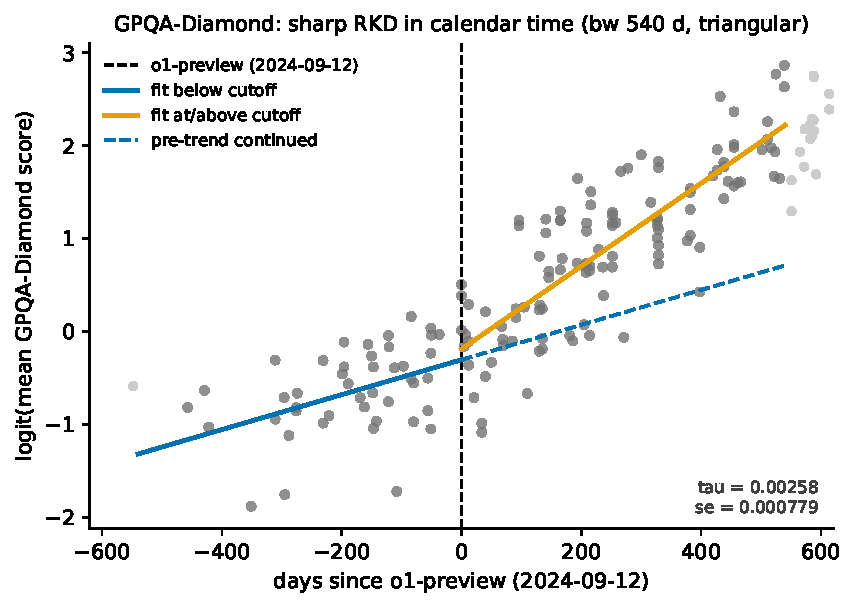
\includegraphics[width=0.66\linewidth]{../../paper/figures/fig_gpqa}
\caption{GPQA-Diamond, logit(mean score) against days since o1-preview
(reproduced from \cite{flagship}): per-side local-linear fits (bandwidth 540
days) versus the continued pre-trend; placebo empirical size 0/7.}
\label{fig:gpqa}
\end{figure}

\section{A sharp bend, no verdict: US adoption at DeepSeek-R1}\label{sec:btosr1}

The project's flagship adoption analysis ends in an instructive split
verdict \cite{notebtosr1}. In the BTOS sector panel (20 sectors $\times$ 54
biweekly waves), a sector-by-wave DiD scan localizes an acceleration in
AI-exposed sectors (information; finance; professional services) at
$t_0=2025.089$ --- \emph{exactly} the first survey wave after DeepSeek-R1's
release on 2025-01-20 \cite{guo2025} --- with scan $p=0.010$--$0.030$; the
exposed-minus-unexposed gap slope more than triples ($+4.2 \to +13.9$
pp/yr), and the group DiK at the release date is nominally significant
($+7.30$ pp/yr, CR1 se $2.80$, $|t|=2.61$). The localization survives
composition checks and placebo-in-space (0/13 pseudo-treated control
sectors). But attribution to R1 fails five ways: placebo cutoffs at
non-event dates return DiKs as large or larger ($+11.4$ pp/yr at $t=2024.30$,
$|t|=3.21$; $+4.0$ at $2024.50$, $|t|=4.53$); only 2/6 specification
variants at R1 are significant; equally large local kinks appear in
non-exposed sectors (real estate, arts, health care); the predicted
\emph{deceleration} at o1 sign-flips with bandwidth; and the cutoff week is
confounded --- the AI-diffusion export rule (2025-01-13), the Stargate
announcement (2025-01-21), and a BTOS sample-year rollover in mid-December
2024 all sit inside the window. The verdict of record: something bent US
business AI adoption in January 2025, and the localization is data-driven
--- but these data cannot say it was R1 (Figure~\ref{fig:btosr1}).

\begin{figure}[t]
\centering

\includegraphics[width=0.9\textwidth]{../btos-sector-did-r1/figures/fig1}
\caption{Adoption at R1 (reproduced from \cite{notebtosr1}): (a) BTOS
AI-use share by exposure group with o1 and R1 marked; (b) group-DiK
estimates at R1, o1, and four non-event placebo dates --- two placebos are
significant, one larger than the R1 estimate.}
\label{fig:btosr1}
\end{figure}

\section{Sycophancy did not win votes --- and the rollback isn't what it looks like}\label{sec:lmarena}

The GPT-4o sycophancy episode of April 2025 \cite{openai2025a} supplies the
corpus's only deploy-and-rollback interrupted time series, inside 135,634
LMArena battles \cite{notelmarena}. The \emph{deploy} leg is credible: the
live 4o alias shows a sharp markdown-style collapse timed to April 25--26
(headers per 1k tokens $3.52 \to 1.12$; sliding-cut permutation $p=0.0128$,
rank 1/78) while nine pinned dated snapshots stay flat --- proving the arena
copy was not pinned --- and it delivers a precise null on the headline
mechanism: the Bradley--Terry-adjusted win-rate change during the sycophancy
window is $+0.02$ log-odds (SE $0.14$; implied win rate $0.540 \to 0.545$).
During the four days users saw the sycophantic build, it gained zero
opponent-adjusted votes --- a clean behavioral null on the
preference-hacking mechanism the literature predicted \cite{sharma2024}. The
\emph{rollback} leg is an identified artifact: on exactly 2025-04-29 the
pinned \texttt{claude-3-7-sonnet-20250219} snapshot --- whose weights cannot
change --- takes an equal-and-opposite persistent step in style \emph{and}
BT strength ($-0.54$ log-odds), demonstrating an arena-side serving change
that contaminates every 29-April estimate. The 4o post-rollback regime never
reverts (the episode is A--B--C, not A--B--A), and the widely repeated
``sycophancy raised the win rate, rollback lowered it'' narrative loads
entirely on the confounded boundary. Pinned snapshots are the cheap,
decisive placebo for platform time series (Figure~\ref{fig:lmarena}).

\begin{figure}[t]
\centering

\includegraphics[width=0.84\textwidth]{../lmarena-sycophancy-aba/figures/fig1}
\caption{The deploy--rollback episode (reproduced from \cite{notelmarena}):
(a) daily bold-markers per 1k tokens for 4o, the pinned \texttt{claude-3-7}
control, and pooled pinned snapshots --- the pinned control steps,
mirror-imaged, on exactly the rollback date; (b) 4o Bradley--Terry strength
by segment: the deploy jump is $+0.02$ log-odds.}
\label{fig:lmarena}
\end{figure}

\section{An identified inference artifact: hyperscaler capex at ChatGPT}\label{sec:capex}

The capex analysis is included as a first-class finding precisely because
its battery caught the failure mode that would otherwise headline this
literature \cite{notecapex}. Big-4 hyperscaler capital expenditure (EDGAR
XBRL reconstruction) accelerates against a six-firm non-AI capital-intensive
aggregate after ChatGPT: group DiK $+0.1396$ dex/yr (HC1 se $0.0302$,
nominal $p=3.9\times10^{-6}$), positive in 18/18 specification cells,
localized over 2023.0--2023.5 exactly as a lagged investment response would
be, and visible per firm for Microsoft, Alphabet, and Amazon but null for
Meta. Every conventional robustness check passes. What kills the causal
reading is the clean pre-period placebo grid: at 15 non-event cutoffs in
2017--2020 the identical specification rejects at nominal 5\% seven times
(empirical size $0.47$), the largest placebo $|z|$ ($5.11$, at 2019.75)
exceeds the ChatGPT estimate's matched-bandwidth $|z|$ ($4.35$), a
full-sample kink at the non-event date 2021.5 reaches $|z|=6.9$, and the BIS
export-control date eight weeks earlier is statistically indistinguishable
($+0.125$, $z=4.0$). Placebo-calibrated, the ChatGPT estimate's $p$ is
$0.125$--$0.25$: the nominal $p$-value overstates the evidence by five
orders of magnitude, because HC1 inference assumes serial independence and
the residual lag-1 autocorrelation reaches $0.66$
\cite{bertrand2004}. The slope divergence is a genuine, robust data feature;
the ``significance'' was an artifact of the standard errors, and only the
battery could tell the two apart (Figure~\ref{fig:capex}).

\begin{figure}[t]
\centering

\includegraphics[width=0.9\textwidth]{../capex-dik-chatgpt/figures/fig1}
\caption{Capex at ChatGPT (reproduced from \cite{notecapex}): (a) quarterly
capex of the big-4 and control aggregates with the BIS and ChatGPT dates
marked; (b) DiK estimates at 15 pre-period non-event placebo cutoffs versus
ChatGPT --- seven placebos reject, and the largest placebo $|z|$ exceeds the
ChatGPT $|z|$.}
\label{fig:capex}
\end{figure}

\section{An honest null with power: the ECI at o1, fresh vintage}\label{sec:ecifresh}

If ``everything kinked in 2024,'' the per-benchmark results of
Section~\ref{sec:gpqa} would be uninformative; the Epoch Capabilities Index
(ECI) \cite{ho2025} is the aggregate guard, and it holds on a fresh vintage
with twelve more months of data \cite{noteeci,flagship}. The all-models
RKD-in-time at o1-preview is $+0.0065$ ECI points/day (se $0.0131$,
$t=0.50$, $p=0.62$; slopes $\approx 22.3$ vs.\ $24.7$ points/yr), null in
17/18 grid cells --- while the same specification rejects at 4/8 placebo
cutoffs elsewhere in the series: the instrument demonstrably moves, and
reads zero at the release date. The vintage's one new nominally significant
result is itself a triage exhibit: a precision-weighted rerun (weights
$1/\sigma_i^2$ from published CIs) returns a negative kink significant in
18/18 cells ($-0.0190$, $p=0.016$) --- which the battery identifies as
smooth post-2024 concavity, not an o1-localized break, because placebo
cutoffs at $+90$/$+180$ days give same-sign \emph{larger} kinks ($-0.0399$,
$p=0.0064$; $-0.0297$, $p=5.5\times10^{-6}$) and a local quadratic absorbs
it ($p=0.14$). A tempting third series --- strict frontier records --- is a
non-design (4 pre-cutoff points in the estimation cell; its nominal
$t=2.28$ dies under a 30-day donut and flips sign under a 45-day one).
Whatever the reasoning-model recipe did to AI capabilities, it did not bend
the aggregate index's calendar-time trend at the release date
(Figure~\ref{fig:eci}).

\begin{figure}[t]
\centering

\includegraphics[width=0.9\textwidth]{../eci-fresh-kink-o1/figures/fig1}
\caption{The ECI null (reproduced from \cite{noteeci}): (a) 211 fresh-vintage
ECI scores against days since o1-preview with unweighted and CI-weighted
per-side fits; (b) kink estimates at the o1 cutoff and eight placebo
cutoffs, both weightings --- the unweighted design rejects at 4/8 placebos
while reading zero at o1.}
\label{fig:eci}
\end{figure}

\section{Coverage: everything considered}\label{sec:coverage}

The survey claim rests on Tables \ref{tab:studied} and \ref{tab:excluded}:
every dataset--design pair the project considered, with its verdict or its
reason for exclusion. Beyond the eight findings above, the studied set
includes the flagship graveyard \cite{flagship} --- a $t=12.9$
``kink'' in cumulative GPU-cluster stock at ChatGPT that fails \emph{every}
placebo (empirical size 7/7: smooth super-exponential curvature bends
everywhere), a sign-unstable Chinchilla null, and the EU threshold correctly
rejected as a kink because it is a step with sorting --- plus a blind LoRD3
scan that missed Chinchilla's adoption ramp and correctly diagnosed its own
top discovery as a fine-tune measurement artifact \cite{notechinchilla},
and a financial-series stress test in which every ``credible'' automated
verdict on semiconductor stocks dissolved under inspection --- the DeepSeek
``kink'' (Holm $p=1.4\times10^{-8}$) is the 2025 AI rally sitting on both
sides of a one-week crash \cite{notesemis}.

\begin{table}[p]
\centering
\footnotesize
\setlength{\tabcolsep}{4pt}
\caption{Studied to verdict: the 17 dataset--design analyses of record.}
\label{tab:studied}
\begin{tabular}{@{}p{0.31\linewidth}p{0.24\linewidth}p{0.30\linewidth}p{0.075\linewidth}@{}}
\toprule
Data $\times$ design & Cutoff / event & Verdict & Ref.\ \\
\midrule
GPQA-Diamond logit scores $\times$ RKD-in-time & o1-preview 2024-09-12 &
credible, date-localized (placebo 0/7) & \cite{flagship} \\
METR 50\% time horizon $\times$ RKD-in-time & o1-preview &
era bend real; date attribution fails (pre-side placebos 3/6) & \cite{flagship} \\
ECI 2025 vintage $\times$ RKD-in-time & o1-preview &
null with power (falsification guard) & \cite{flagship} \\
ECI fresh vintage, unweighted / CI-weighted / frontier records $\times$ RKD &
o1-preview & null upgraded; weighted ``kink'' $=$ curvature artifact;
records series non-estimable & \cite{noteeci} \\
China vs.\ hyperscaler chip stocks $\times$ group DiK (legal; total incl.\
smuggled) & controls 2023-10-17 & credible ($-0.3$ to $-0.56$ ln/yr);
total attenuated and fragile & \cite{noteexport} \\
Country panel, $\geq 10^{24}$-FLOP run counts $\times$ SuDDDS DiD + SC/GESS &
controls 2022Q4 & descriptive-only (placebo-in-space exact $p=1.0$) &
\cite{noteexport} \\
BTOS sector panel $\times$ group DiK + SuDDDS scan & DeepSeek-R1 2025-01-20 &
descriptive-only; attribution fails triage & \cite{notebtosr1} \\
BTOS national spliced series $\times$ measurement RDiT + blind LoRD3 &
rewording, wave 202524 & credible; splice factor $+6.04$ pp / $1.553$ &
\cite{notereword} \\
EDGAR capex panel $\times$ group DiK & ChatGPT 2022-11-30 &
descriptive-only; nominal inference identified as artifact & \cite{notecapex} \\
LMArena battles $\times$ ABA ITS + windowed Bradley--Terry & deploy
2025-04-25, rollback 04-29 & deploy leg credible (vote null); rollback leg
identified arena-side artifact & \cite{notelmarena} \\
Epoch compute panel $\times$ binned-Poisson bunching + Fisher contrasts &
EU AI Act $10^{25}$ FLOP, 2024-08-01 & credible (moderate): bunching,
behavioral or reporting & \cite{noteeuact} \\
EU AI Act threshold $\times$ kink/RD probes & $10^{25}$ FLOP &
rejected: step with sorting, wrong estimand shape & \cite{flagship} \\
GPU-cluster cumulative stock $\times$ RKD-in-time & ChatGPT &
rejected: placebo size 7/7 on super-exponential series & \cite{flagship} \\
Tokens-per-parameter $\times$ RKD-in-time & Chinchilla 2022-03-29 &
sign-unstable null & \cite{flagship} \\
Tokens-per-parameter $\times$ blind LoRD3 scan & (discovery) & honest miss:
top discovery is a fine-tune measurement artifact, correctly diagnosed &
\cite{notechinchilla} \\
Semiconductor weeklies $\times$ kinks, RDD, DiD scan & BIS rounds; DeepSeek
week & all ``credible'' verdicts artifacts of trend regimes; informative DiD
null & \cite{notesemis} \\
ADH Prop-99 panel $\times$ blind SuDDDS + synthetic control & 1989 &
benchmark recovered exactly (validation anchor) & \cite{noteprop99} \\
\bottomrule
\end{tabular}
\end{table}

\begin{table}[t]
\centering
\footnotesize
\setlength{\tabcolsep}{4pt}
\caption{Considered and excluded: 15 candidate pairs with reasons of record.}
\label{tab:excluded}
\begin{tabular}{@{}p{0.46\linewidth}p{0.49\linewidth}@{}}
\toprule
Candidate pair & Reason excluded \\
\midrule
DCM inference-price series $\times$ kink at DeepSeek-V3 & series ends
2025-02 with five flat terminal months: no post-slope identifiable \\
Epoch cyber-vulnerabilities $\times$ post-reasoning event study & no
processed dataset exists (the published download is the raw CVE git
repository) \\
BTOS state panel $\times$ Bartik-style DiD & requires external ACS/BLS
exposure weights; $\sim$40\% of state-level cells disclosure-suppressed \\
R\&D input-share table $\times$ any family & $n=7$ rows; no
quasi-experimental design applies \\
GPQA/METR o1 kinks; China DiK $\times$ standalone mini-papers & already
results of record in \cite{flagship}; duplication adds nothing \\
GPU-cluster / datacenter cumulative growth $\times$ standalone kink
mini-paper & already rejected in the flagship graveyard (placebo empirical
size 1.0: curvature, not kink); no standalone treatment \\
Chip sales + components $\times$ chip-level SuDDDS at the Apr-2025 H20
license round & needs a shared chip-alias map and ragged-2026 panel
preparation; strongest queued follow-up \\
Datacenter site-level panel $\times$ SuDDDS at Colossus/Stargate entry &
18\% of timeline rows are unflagged projections requiring filtering; queued \\
LMArena leaderboard history $\times$ RKD around model-spec releases &
cumulative Bradley--Terry ratings are serially cumulative series; the
GPU-cluster placebo failure is the direct precedent \\
LMArena style-premium DiD around Model Spec / constitution updates &
spec-with-model-update confound requires judge-score validation not yet
run \\
AI-company revenue/WAU $\times$ kink at ChatGPT & zero pre-cutoff mass at
the treatment date; not formalizable \\
Polling cross-section $\times$ threshold RDs (income step, age cliff) &
single survey wave; no microdata, sample sizes, or field dates \\
Values-in-the-wild / CCAI votes $\times$ any design & one aggregate
snapshot; no behavioral treatment channel \\
Benchmark panel $\times$ teaching-to-the-test DEE with IRT difficulties &
requires a 52-benchmark IRT panel build; queued \\
All-models panel $\times$ bunching at $10^{26}$ FLOP (US EO line) +
disclosure-as-outcome scan & only 3 models ever above the line; no
identifiable density contrast \\
\bottomrule
\end{tabular}
\end{table}

\section{Discussion}\label{sec:discussion}

\paragraph{The scoreboard.} Of 17 analyses carried to verdict, four
estimates survive as credible (the rewording jump, the legal-channel export
bend, the GPQA kink, and --- graded moderate --- the EU-Act bunching), two
nulls carry power certificates (ECI at o1, twice; the LMArena vote null),
and at least six nominally significant results were killed or reclassified
by the battery: the R1 attribution, the capex kink, the CI-weighted ECI
kink, the datacenter $t=12.9$, the semiconductor ``kinks'' at three
cutoffs, and the LMArena rollback narrative. That kill rate --- roughly half
of everything that would have cleared a naive $p<0.05$ bar --- is the
central empirical fact of the survey.

\paragraph{Nominal inference on the public record of AI is broken by
default.} The corpus's series are short, serially dependent, and smooth;
HC1/CR1 standard errors on them manufacture $|z|>6$ at dates where nothing
happened (capex at 2021.5; datacenters everywhere; the DeepSeek rally
kink). Placebo calibration measures the size distortion directly --- a
nominal 5\% test rejecting 47\% of the time in the capex pre-period --- and
is cheap. Every headline in this literature should be read against a
placebo distribution or not at all \cite{ganong2018,bertrand2004}.

\paragraph{Era bends are not event bends, and calendar weeks are crowded.}
The shifted-cutoff grid mechanically separates ``the trend changed in this
era'' (METR, the January-2025 adoption surge) from ``this event changed the
trend'' (GPQA, the rewording). Even when a bend localizes, the week is
shared: R1 sits with the diffusion rule, Stargate, and a panel rollover;
ChatGPT sits eight weeks from the BIS controls; the export-control kink is
localized only to $\pm 1$ quarter. Date-localization is necessary, never
sufficient, for attribution.

\paragraph{Measurement is a treatment.} The single largest causal effect in
the corpus --- $+6$ pp of ``AI adoption'' overnight --- was produced by a
questionnaire. The EU-Act deficit may partly be labs' disclosure behavior
rather than training behavior; the BTOS rollover shifts respondent
composition; LMArena's serving configuration moved a pinned model.
Instrument changes mimic adoption, compliance mimics avoidance, and
platform operations mimic model behavior; designs on the public record need
measurement-side placebos (pinned controls, sibling instruments, archived
outcomes) as much as treatment-side ones.

\paragraph{Nulls and refusals are results.} The ECI null is informative
because the same specification rejects at 4/8 placebo cutoffs --- the dial
works and reads zero. The LMArena null is informative because the style
break proves the treatment arrived. And the pipeline's refusals (NaN rather
than a number when placebo pools are too small) repeatedly prevented
fabricated certainty. An automated discovery stack earns trust not by what
it finds but by what it declines to claim; the blind Prop-99 recovery, the
blind re-localization of the rewording cutoff, and the honestly diagnosed
Chinchilla miss are the same machinery validated, confirming, and
self-correcting.

\emph{Limitations.} Calendar-time designs rest on an untestable
no-co-located-event assumption that placebo grids probe but cannot certify.
Several verdicts lean on few units (4 country groups, 7 sector clusters, 6
quarterly points per cell) where all asymptotic inference is optimistic.
Epoch compute figures are partly estimates; benchmark contamination drifts;
and every capability result is a property of the release stream, not of
individual systems. The survey covers the public record through mid-2026;
the queued designs in Table~\ref{tab:excluded} continue it.

\subsection*{Reproducibility}

All estimates were produced with the open-source \natex{} toolkit
\cite{natex} (v0.2.0, seeds declared per note) from public data that are
never committed to the repository. Every figure in this paper is reused
verbatim from a companion note's committed figure, and each of those
figures regenerates deterministically from a script that asserts the
quoted headline numbers against the analysis records before drawing. The
companion notes
\cite{flagship,notereword,noteexport,notebtosr1,notecapex,notelmarena,noteeuact,noteeci,notechinchilla,noteprop99,notesemis}
carry the full specification grids, placebo batteries, and
honest-inference notes summarized here.

\scriptsize
\begin{multicols}{2}
\raggedright
\begin{thebibliography}{99}
\setlength{\itemsep}{1pt}\setlength{\parskip}{0pt}

\bibitem{abadie2021}
Abadie, A. (2021).
Using synthetic controls: Feasibility, data requirements, and methodological
aspects.
\emph{Journal of Economic Literature}, 59(2), 391--425.

\bibitem{abadie2010}
Abadie, A., Diamond, A., and Hainmueller, J. (2010).
Synthetic control methods for comparative case studies: Estimating the effect
of California's tobacco control program.
\emph{Journal of the American Statistical Association}, 105(490), 493--505.

\bibitem{abadie2015}
Abadie, A., Diamond, A., and Hainmueller, J. (2015).
Comparative politics and the synthetic control method.
\emph{American Journal of Political Science}, 59(2), 495--510.

\bibitem{abadiegardeazabal2003}
Abadie, A., and Gardeazabal, J. (2003).
The economic costs of conflict: A case study of the Basque Country.
\emph{American Economic Review}, 93(1), 113--132.

\bibitem{acemoglu2025}
Acemoglu, D. (2025).
The simple macroeconomics of AI.
\emph{Economic Policy}, 40(121), 13--58.

\bibitem{allen2026}
Allen, J.~S. (2026).
Monitoring AI adoption in the U.S. economy.
\emph{FEDS Notes}, Board of Governors of the Federal Reserve System, 3 April
2026.

\bibitem{allen2022}
Allen, G.~C. (2022).
Choking off China's access to the future of AI.
Center for Strategic and International Studies (CSIS), October 2022.
\url{https://www.csis.org/analysis/choking-chinas-access-future-ai}

\bibitem{benmichael2021}
Ben-Michael, E., Feller, A., and Rothstein, J. (2021).
The augmented synthetic control method.
\emph{Journal of the American Statistical Association}, 116(536), 1789--1803.

\bibitem{bernal2017}
Lopez Bernal, J., Cummins, S., and Gasparrini, A. (2017).
Interrupted time series regression for the evaluation of public health
interventions: a tutorial.
\emph{International Journal of Epidemiology}, 46(1), 348--355.

\bibitem{bertrand2004}
Bertrand, M., Duflo, E., and Mullainathan, S. (2004).
How much should we trust differences-in-differences estimates?
\emph{The Quarterly Journal of Economics}, 119(1), 249--275.

\bibitem{besiroglu2024}
Besiroglu, T., Erdil, E., Barnett, M., and You, J. (2024).
Chinchilla scaling: A replication attempt.
arXiv:2404.10102.

\bibitem{bick2026}
Bick, A., Blandin, A., Deming, D., Fuchs-Sch\"undeln, N., and Jessen, J.
(2026).
Measuring AI adoption among firms: How you ask matters.
Federal Reserve Bank of St.\ Louis, \emph{On the Economy}, June 2026.

\bibitem{bockerman2025}
B\"ockerman, P., Jysm\"a, S., and Kanninen, O. (2025).
\emph{Difference-in-Kinks Design}.
IZA Discussion Paper No.~18313.
\url{https://docs.iza.org/dp18313.pdf}

\bibitem{bonney2024}
Bonney, K., Breaux, C., Buffington, C., et al. (2024).
Tracking firm use of AI in real time: A snapshot from the Business Trends and
Outlook Survey.
NBER Working Paper No.~32319.

\bibitem{bonney2026}
Bonney, K., Breaux, C., Dinlersoz, E., et al. (2026).
The microstructure of AI diffusion: Evidence from firms, business functions,
and worker tasks.
Census Bureau CES Working Paper CES-WP-26-25; NBER Working Paper No.~35141.

\bibitem{bown2020}
Bown, C.~P. (2020).
Export controls: America's other national security threat.
Peterson Institute for International Economics Working Paper 20-8.

\bibitem{bradleyterry1952}
Bradley, R.~A., and Terry, M.~E. (1952).
Rank analysis of incomplete block designs: I.\ The method of paired
comparisons.
\emph{Biometrika}, 39(3/4), 324--345.

\bibitem{calonico2014}
Calonico, S., Cattaneo, M.~D., and Titiunik, R. (2014).
Robust nonparametric confidence intervals for regression-discontinuity
designs.
\emph{Econometrica}, 82(6), 2295--2326.

\bibitem{cameron2015}
Cameron, A.~C., and Miller, D.~L. (2015).
A practitioner's guide to cluster-robust inference.
\emph{Journal of Human Resources}, 50(2), 317--372.

\bibitem{card2015}
Card, D., Lee, D.~S., Pei, Z., and Weber, A. (2015).
Inference on causal effects in a generalized regression kink design.
\emph{Econometrica}, 83(6), 2453--2483.

\bibitem{census2025}
U.S. Census Bureau (2025).
\emph{Business Trends and Outlook Survey: AI core question updates}.
3 December 2025.
\url{https://www.census.gov/hfp/btos/downloads/AI\%20Question\%20Wording\%20Updates.pdf}

\bibitem{cheng2025}
Cheng, M., Yu, S., Lee, C., et al. (2025).
Social sycophancy: A broader understanding of LLM sycophancy.
arXiv:2505.13995.

\bibitem{chiang2024}
Chiang, W.-L., Zheng, L., Sheng, Y., et al. (2024).
Chatbot Arena: An open platform for evaluating LLMs by human preference.
\emph{ICML 2024}, PMLR 235:8359--8388.

\bibitem{crosignani2025}
Crosignani, M., Han, L., Macchiavelli, M., and Silva, A.~F. (2025).
Securing technological leadership? The cost of export controls on firms.
Federal Reserve Bank of New York Staff Report No.~1096.

\bibitem{eisfeldt2023}
Eisfeldt, A.~L., Schubert, G., and Zhang, M.~B. (2023).
Generative AI and firm values.
NBER Working Paper No.~31222.

\bibitem{epochdata}
Epoch AI (2026).
Data on AI: AI Benchmarking Hub, Epoch Capabilities Index, and AI chip data.
\url{https://epoch.ai/data}. Retrieved 2026. CC-BY 4.0.

\bibitem{epochchips}
Epoch AI (2026).
Data on AI chip owners.
\url{https://epoch.ai/data/ai-chip-owners} (extract of 2026).

\bibitem{epochmodels}
Epoch AI (2026).
Data on AI models.
\url{https://epoch.ai/data/ai-models} (extract of 2026).

\bibitem{euaiact2024}
European Union (2024).
Regulation (EU) 2024/1689 laying down harmonised rules on artificial
intelligence (Artificial Intelligence Act).
\emph{Official Journal of the European Union}, L series, 12 July 2024.

\bibitem{fichtenberg2000}
Fichtenberg, C.~M., and Glantz, S.~A. (2000).
Association of the California Tobacco Control Program with declines in
cigarette consumption and mortality from heart disease.
\emph{New England Journal of Medicine}, 343(24), 1772--1777.

\bibitem{fist2023}
Fist, T., and Grunewald, E. (2023).
\emph{Preventing AI Chip Smuggling to China: A Working Paper}.
Center for a New American Security (CNAS), October 2023.

\bibitem{ganong2018}
Ganong, P., and J\"ager, S. (2018).
A permutation test for the regression kink design.
\emph{Journal of the American Statistical Association}, 113(522), 494--504.

\bibitem{guo2025}
Guo, D., Yang, D., Zhang, H., et al. (2025).
DeepSeek-R1 incentivizes reasoning in LLMs through reinforcement learning.
\emph{Nature}, 645(8081), 633--638.

\bibitem{han2025}
Han, Z. (2025).
Silicon disruption: An event study of DeepSeek R1's breakthrough impact on
semiconductor markets.
\emph{SHS Web of Conferences}, 218, 01030 (ICDDE 2025).

\bibitem{hausman2018}
Hausman, C., and Rapson, D.~S. (2018).
Regression discontinuity in time: Considerations for empirical applications.
\emph{Annual Review of Resource Economics}, 10, 533--552.

\bibitem{heimkoessler2024}
Heim, L., and Koessler, L. (2024).
Training compute thresholds: Features and functions in AI regulation.
arXiv:2405.10799.

\bibitem{herlands2020}
Herlands, W. (2020).
\emph{Change Modeling for Understanding Our World and the Counterfactual
One(s)}.
PhD thesis, Carnegie Mellon University.

\bibitem{herlands2018}
Herlands, W., McFowland~III, E., Wilson, A.~G., and Neill, D.~B. (2018).
Automated local regression discontinuity design discovery.
In \emph{KDD~'18}.

\bibitem{flagship}
Hillebrandt, H. (2026).
Three kinks and a null: Formal trend-break tests on the public record of AI
progress.
\natex{} paper collection, flagship paper.
\url{https://haukehillebrandt.github.io/natex/paper/}

\bibitem{notebtosr1}
Hillebrandt, H. (2026).
A sharp bend, no verdict: Difference-in-kinks tests of US business AI
adoption at DeepSeek-R1.
\natex{} paper collection, companion note.
\url{https://haukehillebrandt.github.io/natex/btos-sector-did-r1/}

\bibitem{notereword}
Hillebrandt, H. (2026).
The question is the treatment: A known-cutoff regression discontinuity at
the BTOS AI-question rewording.
\natex{} paper collection, companion note.
\url{https://haukehillebrandt.github.io/natex/btos-rewording-rdd/}

\bibitem{notecapex}
Hillebrandt, H. (2026).
A genuine bend, no causal certificate: Difference-in-kinks tests of
hyperscaler capital expenditure at ChatGPT.
\natex{} paper collection, companion note.
\url{https://haukehillebrandt.github.io/natex/capex-dik-chatgpt/}

\bibitem{notechinchilla}
Hillebrandt, H. (2026).
An honest miss: Chinchilla as an adoption ramp in a discontinuity scan of
tokens per parameter.
\natex{} paper collection, companion note.
\url{https://haukehillebrandt.github.io/natex/chinchilla-writeup/}

\bibitem{noteeci}
Hillebrandt, H. (2026).
Still no kink at o1: A precision-weighted rerun of the Epoch Capabilities
Index on a fresh vintage.
\natex{} paper collection, companion note.
\url{https://haukehillebrandt.github.io/natex/eci-fresh-kink-o1/}

\bibitem{noteeuact}
Hillebrandt, H. (2026).
Bunching below the line: Missing mass above the EU AI Act's
$10^{25}$-FLOP threshold.
\natex{} paper collection, companion note.
\url{https://haukehillebrandt.github.io/natex/euact-bunching-writeup/}

\bibitem{noteexport}
Hillebrandt, H. (2026).
Bent, bypassed, unbowed: US AI-chip export controls and China's compute.
\natex{} paper collection, companion note.
\url{https://haukehillebrandt.github.io/natex/export-controls-three-leg/}

\bibitem{notelmarena}
Hillebrandt, H. (2026).
Sycophancy did not win votes: The GPT-4o deploy--rollback episode in
135,634 LMArena battles.
\natex{} paper collection, companion note.
\url{https://haukehillebrandt.github.io/natex/lmarena-sycophancy-aba/}

\bibitem{noteprop99}
Hillebrandt, H. (2026).
Recovering Proposition 99 blind: Validating the \natex{} pipeline against
the Abadie--Diamond--Hainmueller benchmark.
\natex{} paper collection, companion note.
\url{https://haukehillebrandt.github.io/natex/prop99-validation-writeup/}

\bibitem{notesemis}
Hillebrandt, H. (2026).
The rally, not the rule: Semiconductor stocks at the US export controls and
DeepSeek under automated natural-experiment validation.
\natex{} paper collection, companion note.
\url{https://haukehillebrandt.github.io/natex/semis-event-studies-writeup/}

\bibitem{natex}
Hillebrandt, H. (2026).
\emph{natex: automated natural-experiment discovery and estimation} (version
0.2.0). Software.
\url{https://github.com/HaukeHillebrandt/natex}

\bibitem{ho2025}
Ho, A., Denain, J.-S., Atanasov, D., Albanie, S., and Shah, R. (2025).
A Rosetta Stone for AI benchmarks.
arXiv:2512.00193.

\bibitem{hoffmann2022}
Hoffmann, J., Borgeaud, S., Mensch, A., et al. (2022).
Training compute-optimal large language models.
\emph{NeurIPS 2022}. arXiv:2203.15556.

\bibitem{hooker2024}
Hooker, S. (2024).
On the limitations of compute thresholds as a governance strategy.
arXiv:2407.05694.

\bibitem{hu1995}
Hu, T.-W., Sung, H.-Y., and Keeler, T.~E. (1995).
Reducing cigarette consumption in California: Tobacco taxes vs an
anti-smoking media campaign.
\emph{American Journal of Public Health}, 85(9), 1218--1222.

\bibitem{jakubowski2023}
Jakubowski, B., Somanchi, S., McFowland~III, E., and Neill, D.~B. (2023).
Exploiting discovered regression discontinuities to debias
conditioned-on-observable estimators.
\emph{Journal of Machine Learning Research}, 24(133), 1--57.

\bibitem{juniewicz2026}
Juniewicz, I. (2026).
Diversion and resale: Estimating compute smuggling to China.
Epoch AI, April 2026.
\url{https://epoch.ai/publications/chip-smuggling}

\bibitem{kaplan2020}
Kaplan, J., McCandlish, S., Henighan, T., et al. (2020).
Scaling laws for neural language models.
arXiv:2001.08361.

\bibitem{kleven2016}
Kleven, H.~J. (2016).
Bunching.
\emph{Annual Review of Economics}, 8, 435--464.

\bibitem{klevenwaseem2013}
Kleven, H.~J., and Waseem, M. (2013).
Using notches to uncover optimization frictions and structural elasticities:
Theory and evidence from Pakistan.
\emph{Quarterly Journal of Economics}, 128(2), 669--723.

\bibitem{kumarmanning2025}
Kumar, I., and Manning, S. (2025).
Trends in frontier AI model count: A forecast to 2028.
arXiv:2504.16138.

\bibitem{kwa2025}
Kwa, T., West, B., Becker, J., et al. (2025).
Measuring AI ability to complete long tasks.
arXiv:2503.14499.

\bibitem{mackinlay1997}
MacKinlay, A.~C. (1997).
Event studies in economics and finance.
\emph{Journal of Economic Literature}, 35(1), 13--39.

\bibitem{mccrary2008}
McCrary, J. (2008).
Manipulation of the running variable in the regression discontinuity design:
A density test.
\emph{Journal of Econometrics}, 142(2), 698--714.

\bibitem{mcelheran2024}
McElheran, K., Li, J.~F., Brynjolfsson, E., et al. (2024).
AI adoption in America: Who, what, and where.
\emph{Journal of Economics \& Management Strategy}, 33(2), 375--415.

\bibitem{miller2022}
Miller, C. (2022).
\emph{Chip War: The Fight for the World's Most Critical Technology}.
Scribner, New York.

\bibitem{openai2024}
OpenAI (2024).
OpenAI o1 System Card.
arXiv:2412.16720.

\bibitem{openai2025a}
OpenAI (2025).
Sycophancy in GPT-4o: What happened and what we're doing about it.
Blog post, 29 April 2025.
\url{https://openai.com/index/sycophancy-in-gpt-4o/}

\bibitem{openai2025b}
OpenAI (2025).
Expanding on what we missed with sycophancy.
Blog post, 2 May 2025.
\url{https://openai.com/index/expanding-on-sycophancy/}

\bibitem{polivka1998}
Polivka, A.~E., and Miller, S.~M. (1998).
The CPS after the redesign: Refocusing the economic lens.
In \emph{Labor Statistics Measurement Issues}, 249--289. U.\ Chicago Press.

\bibitem{rein2023}
Rein, D., Hou, B.~L., Stickland, A.~C., et al. (2023).
GPQA: A graduate-level Google-proof Q\&A benchmark.
arXiv:2311.12022.

\bibitem{saez2010}
Saez, E. (2010).
Do taxpayers bunch at kink points?
\emph{American Economic Journal: Economic Policy}, 2(3), 180--212.

\bibitem{sardana2024}
Sardana, N., Portes, J., Doubov, S., and Frankle, J. (2024).
Beyond Chinchilla-optimal: Accounting for inference in language model
scaling laws.
\emph{ICML 2024}, PMLR 235, 43445--43460.

\bibitem{sastry2024}
Sastry, G., Heim, L., Belfield, H., et al. (2024).
Computing power and the governance of artificial intelligence.
arXiv:2402.08797.

\bibitem{sevilla2022}
Sevilla, J., Heim, L., Ho, A., et al. (2022).
Compute trends across three eras of machine learning.
\emph{IJCNN 2022}.

\bibitem{sharma2024}
Sharma, M., Tong, M., Korbak, T., Duvenaud, D., et al. (2024).
Towards understanding sycophancy in language models.
\emph{ICLR 2024}.

\bibitem{touvron2023}
Touvron, H., et al. (2023).
LLaMA: Open and efficient foundation language models. arXiv:2302.13971.

\bibitem{yotzov2026}
Yotzov, I., Barrero, J.~M., Bloom, N., et al. (2026).
Firm data on AI.
NBER Working Paper No.~34836.

\end{thebibliography}
\end{multicols}

\end{document}
